\documentclass[defaultstyle,12pt]{thesis}
\usepackage{apa} 
\usepackage{times}
\usepackage{graphicx}
\usepackage{url}

%%%%%%%%%%%%%%%%%%%%%%%%%%%%%%%%%%%%%%%%%%%%%%%%%%%%%%%%%%%%%%%%%%%%%%%%%%
% Front matter
%%%%%%%%%%%%%%%%%%%%%%%%%%%%%%%%%%%%%%%%%%%%%%%%%%%%%%%%%%%%%%%%%%%%%%%%%%
\title{What happens next versus when ``next'' happens: \\ Dissociating spatial and temporal prediction mechanisms}
\author{Dean R.}{Wyatte}
\otherdegrees{B.S., Indiana University Bloomington, 2007 \\
M.A., University of Colorado Boulder, 2010}
\degree{Doctor of Philosophy}{Ph.D., Cognitive Neuroscience}
\dept{Department of}{Psychology and Neuroscience}
\advisor{Prof.}{Randall C. O'Reilly}
\reader{Prof.~Tim Curran}	
\readerThree{Prof.~Albert Kim}		%  3rd person to sign thesis
%\readerFour{Mr.~Alfred Remington}	%  4rd person to sign thesis
%%%%%%%%

%%%%%%%%%%%%%%%%%%%%%%%%%%%%%%%%%%%%%%%%%%%%%%%%%%%%%%%%%%%%%%%%%%%%%%%%%%
% Abstract
%%%%%%%%%%%%%%%%%%%%%%%%%%%%%%%%%%%%%%%%%%%%%%%%%%%%%%%%%%%%%%%%%%%%%%%%%%
\abstract{  \OnePageChapter
}
\SuspendPrologue % turn this off until the actual thesis
%%%%%%%%


% From program reqs: Typically the proposal will include introduction, methods, and preliminary results for any completed experiments; along with methods, 
%	hypotheses, and predictions for planned experiments.


% Outline
%
% Introduction 1-2 pages
% * Chief question: World contains rich temporal structure -- how does the brain leverage it to predict what happens following a given input?
%	Specifically in the context of object recognition -- and interestingly, missing from most models (except for trace rule which is sometimes used)
%		* Recent evidence suggests that an unsupervised temporal learning forms invariance -- work from DiCarlo and colleagues
%	No mechanism specified for temporal learning (trace rule is computational account)
%
% * Recent work from our lab developing theoretical and formal models of how this learning takes places.
% 	VERY HIGH LEVEL description of generic TI framework, which maps computational ideas of the SRN onto the biology of the brain, used for many models
% 	Key idea is that t and t+1 are represented in same neural tissue (check TI page for best wording on this), and learn based on this temporal structure
%	Requires memory trace or context to integrate t and t+1, ideally with fixed update interval which we think literature suggests is alpha freq
%
% * Core prediction is that alpha creates perceptual windows of high excitability that can be linked together via TI mechanisms (prediction/context)
%	Rich literature on predictability in vision (either explicitly researching this issue, or is implicitly related), but nothing linked to alpha  (except for one experiment)
%	Dissertation will test in what way alpha is related to predictability and its role in object representations over time

% Background 
% * TI detailed description and Relevant alpha oscillation literature (relevant issues: spatial, temporal attention, modulation by attention, entrainment)
% * Review of relevant behavioral literature -- representational momentum and 3D object recognition and how alpha relates to them

% Potential experiments
% Expt 1: Leverage representational momentum paradigm to test effects of spatial/temporal predictability (same different probe task). Record EEG, analyze alpha
%			Potential modifications on Expt 1 (and future expos if it works out): Role of spatial or divided attention (i.e., left vs right display with valid/invalid cue)
%				-- alpha effects shown to be stronger for unattended hemifield, more "discretized"
%				-- resets with sounds/flash (or flash lag effect) and their effect on RM -- no one has done this with EEG, surprisingly, just showed that there are effects of sounds/flash.
%					unclear what effect is on alpha
%
% Expt 2: More complex objects. Begin to tap recognition question  -- start with faces, which have a robust EEG response. Same basic paradigm as in expt 1. Question is does spatial/temporal
%		predictability modulate dynamic face recognition? Don't expect representational displacement like in expt 1, but could screw with representations of at-threshold faces. Can also do inversion paradigm (paper on
%		this somewhere in papers lib)
%
% Expt 3: More complex objects, begin to tap learning question -- Morphing experiments that show identities become associated and confused due to alpha entrainment -- but not when spatial/temporal properties are
%		broken and predictability is low
%
% Expt 4: Learning with novel objects: Same paradigm as expo 2-3 but for completely unknown objects. Can do pre-post test to see how effects change.
%
% Other stuff -
% How does spatial/temporal coherence affect robustness to occlusion -- gaussian occluder mask with above manipulations -- can do recognition task too? allows linking in with broad literature on object completion and my previous research
% Role of feedback in prediction -- masking/continuous flash suppression?

% Role of modeling:
%	So, far the experiments are qualitative extensions of the theoretical framework. Modeling to produce quantitative fits is possible, especially with respect to how much spatial/temporal randomization can be tolerated. There is also the issue of predictive coding -- can any of the experiments speak to this?
%
%
%
%
%
%% Exp 1:
%    Standard RM paradigm
%    Predict that alpha is actually temporal + reflects some spatial stuff?
%    All comes down to whether we think temporal and spatial expectations can be separated but are both related to alpha (i.e., prediction can only happen once per cycle)
%		Timing errors on alpha, spatial/object-based errors on gamma?
%    
%Exp 2: 
%    RM but with learnable spatial sequences (as opposed to completely random)
%    Predict that alpha effect increases as sequence is learned (divide expt into two blocks or two days or something)
%    
%Exp3: RM with novel 3D objects -- see if Expt 2 effect translates to depth-rotations of 3D objs
%
% Modifications -- Randy also mentioned trying to get at the predictive coding thing or at least trying to zoom in on a question like the role of prediction and experience within a single alpha cycle
%		mixing stimulus complexity or contrast/attention and expectation with the above manipulations to try to get at this question. Need to read KokRahnevJeheeEtAl12

\begin{document}

% cheap title
\chapter*{What happens next versus when ``next'' happens: \\ Dissociating spatial and temporal prediction mechanisms \\ \vspace{20mm} Dean R.~Wyatte}

\chapter{Introduction}
How does the brain predict what happens from one moment to the next? This is an important question in research on perception across all modalities that is surprisingly often overlooked in the fields of psychology and neuroscience. For example, most experiments are designed to measure evoked responses to a randomly chosen, isolated stimulus under the tacit assumption that response variability is irrelevant noise that should be averaged out across many presentations. Computational models of perceptual processing often operate under similar assumptions in which stimuli are presented as random ``snapshots'' from which some common set of features should be learned to minimize representational variability across presentations (e.g., {\nopcite{SerreOlivaPoggio07,MutchLowe08}; although see \nopcite{Foldiak91}, for a notable exception). These experimental and computational assumptions stand in contrast to the event structure of the physical world, which is deterministic from one moment to the next. 

An equally important question is concerned with how the brain knows when to make its next prediction. Predicting what happens next requires integrating information over some time frame and using the result to drive the actual prediction, but when should integration start? And for how long? Perceptual processing has been shown to undergo temporal fluctuations and in extreme cases, stimuli can be rendered imperceptible if presented during one of these fluctuations (\nopcite{BuschDuboisVanRullen09,VanRullenBuschDrewesEtAl11}; \abbrevnopcite{MathewsonLlerasBeckEtAl11}). Again, many laboratory experiments tend not to be concerned with these temporal fluctuations, as they simply add variability to responses that will average out over a large number of trials and can be mitigated by design decisions such using a fixation cross to denote the start of a trial. Computational models, similarly, often completely ignore time altogether, although recent advances in spiking models of perceptual processing \cite[e.g.,]{MasquelierThorpe07} are beginning to address this issue.

The goal of the proposed work is to begin systematically investigating the neural mechanisms and circuitry related to prediction and temporal integration. Recently, our lab has developed a theoretical framework and general model for describing how these functions are implemented in the brain. This framework, henceforth referred to as \textit{LeabraTI},\footnote{Leabra refers to a general model of learning in the neocortex \protect\cite{OReillyMunakata00,OReillyMunakataFrankEtAl12}; TI to Temporal Integration.} brings together a large number of independent findings from the systems neuroscience literature to describe how multiple interacting mechanisms accomplish prediction and temporal integration in cortex. The fundamental proposal of the LeabraTI theory is that time in the brain is discretized (at least partially) into reference frames that can be associated via general learning mechanisms (e.g., Hebbian and error-driven learning) so that representation of information during one frame can be used to predict what happens during the next. This proposal requires at least two mechanisms: (1.)~A mechanism that establishes reference frames over which information is integrated and, (2.)~A mechanism that generates the actual prediction itself and validates it against what actually happens. 

As will be discussed in detail in Chapter \ref{chap:leabrati}, the LeabraTI theory's proposed mechanisms are suggested to be dissociable, generating signatures at distinct spectral frequencies which can be measured physiologically. The potential dissociability of the spatial and temporal components of prediction establishes a number of immediately testable predictions that will form the experimental component of the proposed work. Chapter \ref{chap:experiments} discusses a line of three experiments and predictions within the the context of the LeabraTI theory. The overall space for experimental investigations is quite large and and the experiments proposed in Chapter \ref{chap:experiments} form just one trajectory through it. Chapter \ref{chap:variants} discusses variants of these experiments that target slightly different aspects of the LeabraTI theory. The proposed experiments should be preferred, as they are more well-defined at present, but the variants may replace one or more of the proposed experiments at the committee's discretion.

\chapter{The \textit{LeabraTI} framework}
\label{chap:leabrati} 

The \textit{LeabraTI} framework is a mechanistic description and general model of how prediction and temporal integration might work in the brain. The general idea is largely compatible with the Simple Recurrent Network (SRN) \cite{Elman90,Servan-SchreiberCleeremansMcClelland91}, an artificial neural network architecture that explicitly represents temporally lagged information in discrete ``context'' units whose activity gets integrated with more current information to predict what happens in the next time step (Figure \ref{fig:srn_circuit}a). This method of copying a contextual representation from an intermediate representation at discrete intervals has proven to be a robust way to leverage error-driven learning to represent latent temporal structure in auditory streams and artificial grammars. In theory, the SRN architecture is a powerful abstraction capable of representing the latent structure of any stimulus that varies systematically over time, making it a good candidate for a general prediction and temporal integration mechanism. In this chapter, I describe how such an architecture might be implemented using biological neural circuitry.

% srn/microcircuit fig
\begin{figure}[hp]
\centering
\begin{tabular}{ll}
a) \\
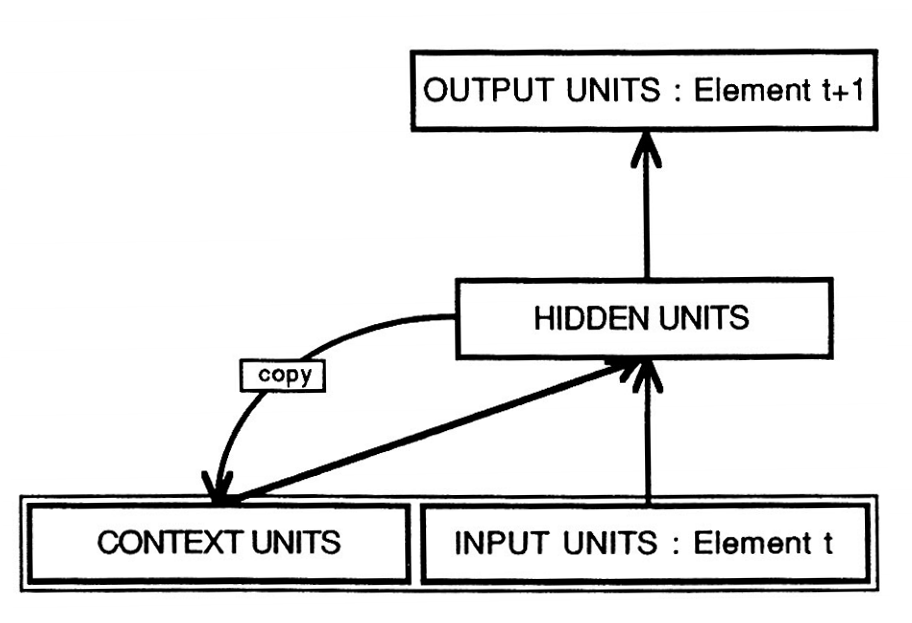
\includegraphics[width=100mm]{srn_scm.png} \\
b) \\
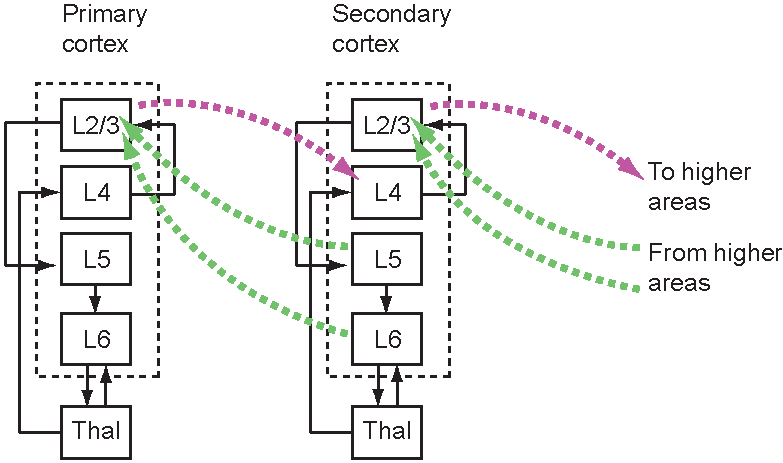
\includegraphics[width=120mm]{microcircuit_horiz.pdf} \\
\end{tabular}
\caption{The Simple Recurrent Network (SRN) and microcircuitry of the neocortex.}
\label{fig:srn_circuit}
\end{figure}

\section{Laminar structure and microcircuitry of the neocortex}
A salient feature of the brain, and potential clue in realizing how an SRN-like computation might be carried out in biological neural circuits, is the laminar structure prevalent across the neocortex. Incoming information from the sensory periphery is transmitted through the thalamus and then enters Layer 4 in the primary sensory cortex (e.g., V1). Cortical areas contain a columnar organization with microcolumns composed of around 100 neurons that   extend vertically through the lamina with a strong degree of isocoding within a given column \cite{Mountcastle97,Jones00,HortonAdams05}. Within the microcolumn exists a canonical circuit with the schematic Layer 4  $\rightarrow$ Layer 2/3 $\rightarrow$ Layer5 $\rightarrow$ Layer 6 that routes spike propagation through the local neuronal structure (Figure \ref{fig:srn_circuit}b).

Despite the strong degree of isocoding within the microcolumn, there exist laminar differences in the response dynamics of neurons. These differences have generally gone underappreciated until recently when studies began employing depth electrodes to simultaneously record from multiple layers within a patch of cortex \cite[e.g.,]{MaierAdamsAuraEtAl10,BuffaloFriesLandmanEtAl11,SpaakBonnefondMaierEtAl12}. This recent work has indicated that superficial layers (Layers 2 and 3) exhibit spectral power at much higher frequencies (gamma spectrum) than deep layers (Layers 5 and 6; alpha spectrum). Examining the laminar microcircuitry reveals why these spectral asymmetries might be present. Specifically, Layers 2 and 4 are a major site of both afferent and efferent synapses between cortical areas \cite{RocklandPandya79}. Deeper layers, in contrast, tend to be more isolated from external interareal inputs and are driven primarily by neurons within the local microcolumn \cite{DouglasMartin04,ThomsonLamy07}. 

The differences in spectral power and connectivity suggest a functional dissociation between superficial and deep layers, which upon closer inspection, actually appear quite compatible with the SRN architecture. The multiple diverging connections from superficial layers allow information to be transmitted downstream for further processing and also recirculated within the local microcolumn,. Within the micrcolumn, the relative isolation of deep layers make them ideal targets for the temporally lagged contextual representation necessary for an SRN-like computation.

\section{Layer 5 rhythmic bursting and contextual gating}
A microcolumn only spans a few millimeters of cortical depth. This relatively small amount of tissue, if driven with continuous input, would circulate spikes at a rate much faster than 10 Hz. How could such a circuit produce the strong alpha power observed in recent depth recordings? Several studies have noted that a subset of Layer 5 neurons exhibit rhythmic bursting in the alpha frequency spectrum \cite{ConnorsGutnickPrince82,SilvaAmitaiConnors91,FlintConnors96,BollimuntaChenSchroederEtAl08}. This rhythmic firing has been shown to persist even with constant sensory stimulation \textit{in vivo} \cite{LuczakBarthoHarris13}, suggesting that Layer 5 neurons' alpha rhythmicity could implement a roughly 10 Hz gating function for spikes relayed to Layer 6 neurons. 

Thus, Layer 6 specifically becomes the neural substrate of the SRN's temporally lagged context representation, representing information that is, on average, one alpha cycle (approximately 100 ms) in the past. This contextual storage occurs at an automatic interval due to the intrinsic pacemaking properties of Layer 5 neurons, and might implement a reference frame that essentially would allow the brain to know \textit{when} to anticipate inputs. As such, intrinsic oscillations have been shown to phase lock to environmental stimulation \cite{LakatosKarmosMehtaEtAl08,SchroederLakatos09}, synchronizing environmental events coincide with key events like Layer 5 bursts in cortex. 

\section{Thalamic gating and prediction in superficial layers}
Layer 6 sends axons toward the thalamus, completing the microcircuit within the local column and allowing the temporally lagged Layer 6 information to integrate with more current Layer 4 inputs. There also exists a direct connection between Layer 6 and Layer 4, that could be used for this purpose, although it has been noted as being weak compared to other intracolumnar connections \cite{HirschMartinez06b}. In either case, temporal associations could be created by simple Hebbian learning mechanisms that track high probability co-occurences across past and present events.

The Leabra algorithm \cite{OReillyMunakata00,OReillyMunakataFrankEtAl12}, however, also makes use of powerful error-driven learning (in addition to more standard Hebbian learning). In the context of temporal integration, error-driven learning wold allow computation of error signals based on the difference between what is predicted to happen at a given moment (given the previous moments context as an input) and what actually happens. However, this computation requires that both the prediction and the actual sensation are represented subsequently within a single alpha cycle, which is not possible if the sensory periphery is always transmitting incoming inputs. To resolve this issue, the LeabraTI framework posits a mechanism to modulate or even block the transmission of inputs from the sensory periphery. A subset of cells in the thalamus exhibit alpha spectrum bursting properties similar to that of Layer 5 neurons (\nopcite{LopesdaSilva91}; \abbrevnopcite{HughesLorinczCopeEtAl04}; \nopcite{LorinczCrunelliHughes08}; \nopcite{LorinczKekesiJuhaszEtAl09}), and thus perhaps perform a similar gating function. Specifically, these neurons appear to shift the balance of inputs to Layer 4 and superficial neurons between exogenous environmental inputs and endogenous inputs local to the microcolumn.

When environmental inputs are downmodulated or blocked, Layer 6 context relayed via the thalamus is the dominant input to the microcolumn, which can be used to predict the incoming sensory event during the latter part of the alpha cycle. Importantly, during both the prediction and sensation phases, feedforward and feedback projections are constantly transmitting between lower and higher cortical areas. As previously mentioned, these projections originate and terminate predominantly in superficial layers, boosting their spike coherence to higher frequency spectra. This could potentially explain the differentially high gamma power in superficial layers compared to deep layers, and provides a compelling link between gamma oscillations and predicting the next sensory event.

\section{Summary of LeabraTI computation}
The overall computation of LeabraTI is shown in Figure \ref{fig:leabrati_comp} and summarized here. When thalamic cells burst (roughly every 100 ms), information from the sensory periphery is the primary driving force for Layer 4 neurons in primary cortex. This information is relayed downstream via the strong feedforward Layer 4 $\rightarrow$ Layer 2/3 $\rightarrow$ Layer 4 pathway \cite{FellemanVanEssen91}. Within the local microcolumn, Layer 5 neurons integrate this information, until thalamic bursting quiets (generally around 50 ms). At this point, Layer 5 cells burst, sending outputs to Layer 6 and shifting and inputs to the microcolumn  endogenously. The information represented by Layer 6 neurons is temporally lagged (from the previous 50 ms) and is relayed to Layer 4 via non-bursting (regular spiking) thalamic neurons or via the direct Layer 6 $\rightarrow$ Layer 4 connection (not pictured in Figure \ref{fig:leabrati_comp}), and might be maintained by reciprocal thalamocortical drive back to Layer 6. This information can be used as a prediction as to what will happen next when thalamic bursting resumes and veridical sensory information serves as the input once again. In the context of Leabra's error-driven learning these two phases correspond to the plus phase (sensation) and minus phase (prediction), which can be used to compute a sensory prediction error signal. This error signal modifies Layer 5 $\rightarrow$ Layer 6 synapses to minimize differences between predictions and sensations over time.

Critically, for the LeabraTI computation to work, thalamic and Layer 5 oscillatory phases need to have an approximately antiphase relationship in order for the error-driven learning scheme described here to work so that Layer 2/3 neurons can represent the current moment's prediction with Layer 6 context as their primary input and then subsequently represent the veridical sensory input while Layer 5 neurons queuing up the next contextual event. Such a relationship has not yet been shown yet, but very few studies have recorded simultaneously from thalamic and cortical neurons in \textit{in vivo} in the awake behaving animal. It is also possible that the brain implements error-driven learning in such a way that does not require representing predictions and sensations temporally interleaved on the same neural substrate or even that the brain accomplishes temporal integration completely without supervision, which in case thalamic gating is not required.

% leabrati computation
\begin{figure}[h]
\centering
\begin{tabular}{ll}
a) \hspace{76mm} b) \\
\multicolumn{2}{c}{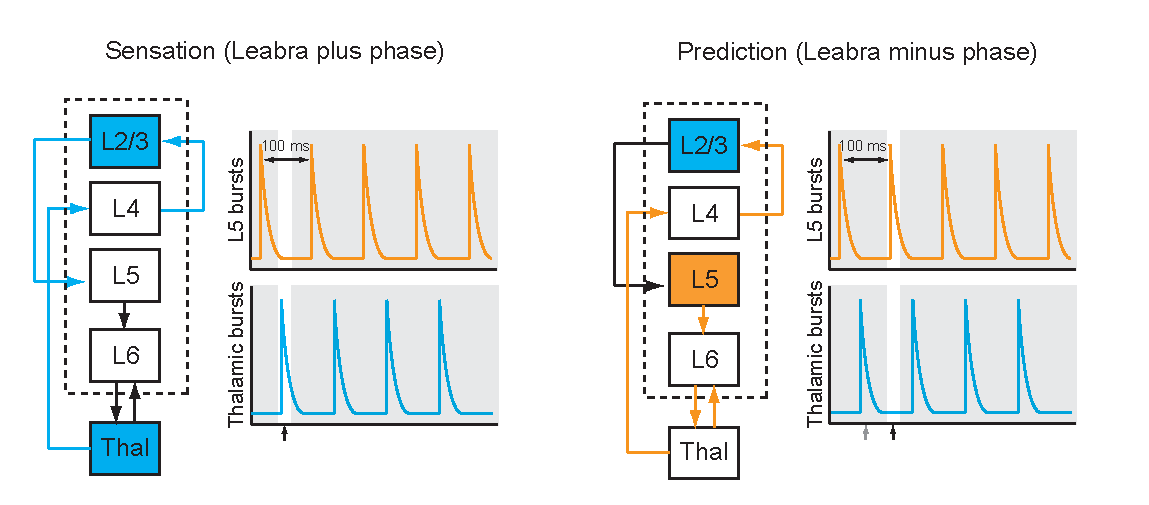
\includegraphics[width=160mm]{leabrati_comp.pdf}} \\
\end{tabular}
\caption{The LeabraTI model computation.}
\label{fig:leabrati_comp}
\end{figure}

\section{Model implementation details and preliminary results}
Thus far, a generic model that embodies the LeabraTI theory has been implemented that can be incorporated into simulations of more specific neural systems (e.g., vision, audition, motor coordination, etc.). The model extends standard Leabra model layers that correspond to superficial-level neurons with a ``deep'' contextual layer containing modifiable synapses in the descending direction, corresponding to the Layer 5 $\rightarrow$ Layer 6 connection in the brain that allows current information to be processed and held onto until the next alpha cycle marked by the Layer 5 neurons' bursts. Ascending synapses are nonplastic and correspond to the Layer 6 transthalamic and/or direct connections to Layer 4 that allows integration of this previous moment's context with more current information. The Layer 4 $\rightarrow$ Layer 2/3 and Layer 2/3 $\rightarrow$ Layer 5 connections are not explicitly modeled and are assumed to operate as a perfect one-to-one relays in the model.

Time in the model is discretized into 100 ms frames coinciding with Layer 5 neurons' alpha spectrum bursting. Each frame contains both Leabra minus and plus phases, with the minus phase driven by deep contextual inputs (no external inputs) and the plus phase driven by the sensory periphery (external inputs), coinciding with thalamic bursting. Full recurrent dynamics are enabled in both phases among superficially connected layers, which are hypothesized to give rise to their differentially high gamma power reported in the literature. Layer 5 context is processed through the Layer 5 $\rightarrow$ Layer 6 synaptic weights at the end of every plus phase in an automatic pacemaker-fashion which is similarly hypothesized to be the mechanism behind deep layers' alpha coherence.

As a proof of concept, this generic LeabraTI model was used to implement a simulation of early visual processing encompassing areas V1 and V2 (Figure \ref{fig:objrec_ti}a). In accordance with standard models of early visual processing, V1 neurons were tuned to oriented Gabors and V2 neurons pooled over the responses of multiple V1 neurons (see \nopcite{OReillyWyatteHerdEtAl13} for specific parameters). Within an area Layer 6 neurons integrated over 3x3 neighborhoods of Layer 5 neurons (relayed from Layer 2/3 neurons), and and sent responses back to Layer 2/3 neurons in a one-to-one manner. Interareal connections encompassing V1 Layer 6 $\rightarrow$ V2 Layer 4 and V2 Layer 6 $\rightarrow$ V1 Layer 2/3 were also included in the model and are consistent with known interareal anatomical connections \cite{RocklandPandya79,ThomsonLamy07}.

% objrec_ti fig
\begin{figure}[h]
\centering
\begin{tabular}{ll}
a) & b) \\
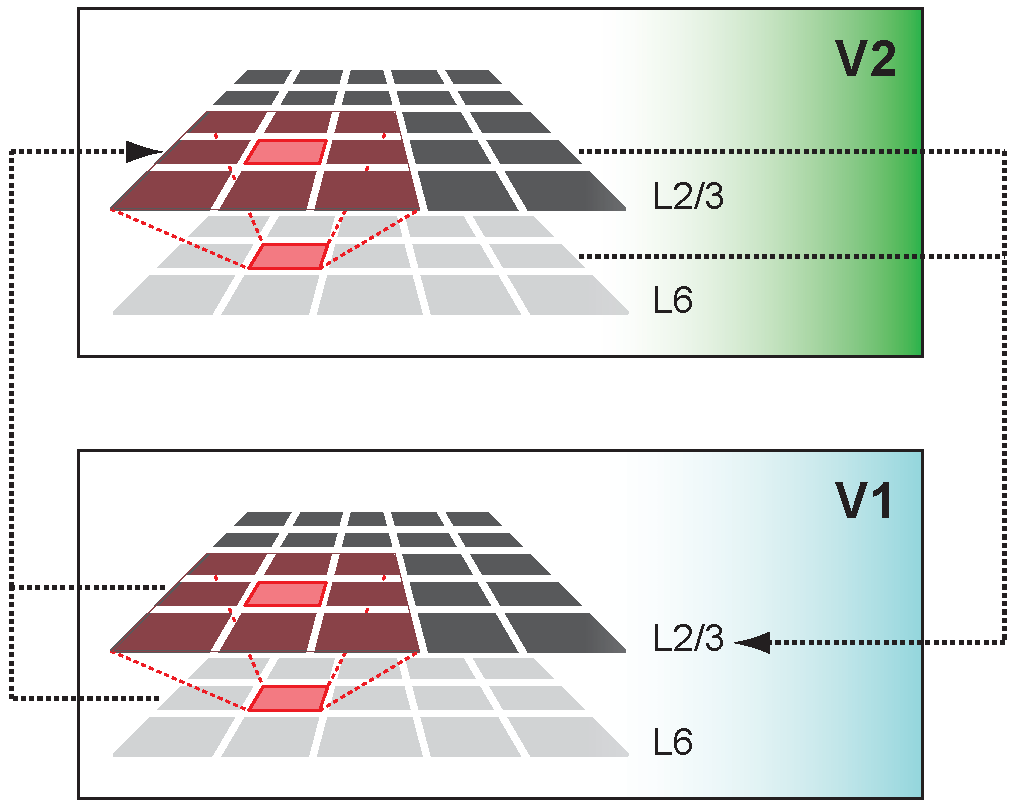
\includegraphics[width=105mm]{leabrati_v1v2.pdf} & 
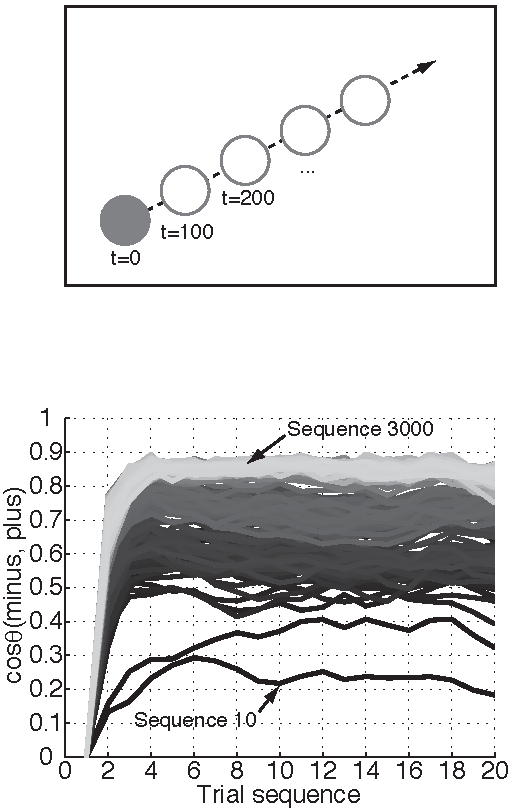
\includegraphics[width=55mm]{sims_v1v2.pdf} \\
\end{tabular}
\caption{LeabraTI implementation in early visual processing encompassing areas V1 and V2.}
\label{fig:objrec_ti}
\end{figure}

The model was shown sequences of stimuli depicting a sphere traveling at a constant velocity in a randomly chosen linear trajectory and sampled this sequence at the beginning of every 100 ms at the start of each trial's plus phase (Figure \ref{fig:objrec_ti}b, top panel). Context was processed through the Layer 5 $\rightarrow$ Layer 6 connections at the end of every plus phase and used to generate the prediction for the following minus phase. Each sequence contained 20 trials, each plus and minus phases. Synaptic weights were modified at the end of each trial using the Leabra XCAL learning rule \cite{OReillyMunakataFrankEtAl12}, which contains both a Hebbian component and an error signal generated from minus-plus phase differences.

Performance on the task was evaluated by computing the cosine (normalized dot product) between Layer 2/3 minus and plus phase responses to determine the distance between predictions and their corresponding sensations. Figure \ref{fig:objrec_ti}b (bottom panel) indicates that the model did a reasonably good job of predicting the sphere's next position from trial-to-trial over the course of 3000 randomly chosen sequences. Importantly the minus-plus cosine metric was significantly greater than a ``null'' prediction which would result in the prediction of the \textit{previous} sphere on the previous trial. This result indicates that the model is indeed learning a genuine predictive code, opposed to a simple reconstructive code. While more analysis will be necessary to characterize the full potential and limitations of the LeabraTI model in the context of more complex tasks, these results suggest that it is at least suitable for well-controlled tasks like the position prediction used here.

\chapter{Background and proposed research}
\label{chap:experiments}

The proposed research is designed to test the LeabraTI theory's central prediction that temporal and spatial prediction mechanisms are dissociable. Specifically, the former is suggested to be subserved by the pacemaking  properties of Layer 5 (and possibly thalamic) neurons' rhythmic bursting that give rise to the brain's alpha rhythm, allowing it know \textit{when} to anticipate inputs. This idea is largely consistent with a large literature suggesting that the alpha rhythm reflects temporal fluctuations in attention (\nopcite{BuschDuboisVanRullen09,VanRullenBuschDrewesEtAl11}; \abbrevnopcite{MathewsonLlerasBeckEtAl11}). Spatial prediction, in contrast, is suggested to depend on prediction-sensation processes, subserved by neural populations in superficial lamina. Activity related to these processes should manifest in the gamma spectrum, as these layers are always active (non-pacemaking) since they are a major site of afferent and efferent interareal synapses.

Surprisingly little work has gone into directly investigating the brain's alpha rhythm in the context of temporal prediction or anticipation. Only one recent paper has directly tested this idea, but there are several related lines of research that are used to motivate the proposed experiments. In their recent paper, \incite{RohenkohlNobre11} manipulated the temporal predictability of a ``ball'' stimulus that traveled across the display in a linear trajectory similar to the simulations in Chapter \ref{chap:leabrati}, except that the ball temporarily disappeared behind an occluder during part of its trajectory. EEG analyses indicated that alpha-band power was correlated with anticipation about when the ball would reappear from behind the occluder, with a higher degree of desynchronization on \textit{rhythmic} (high temporal predictability) compared to \textit{arrhythmic} trials (low temporal predictability).

The results of \incite{RohenkohlNobre11} are somewhat difficult to interpret in the broader context of the LeabraTI theory since it associates different mechanisms with temporal and spatial predictability. In their experiment, temporal predictability of the ball was confounded with spatial predictability, as the ball always traveled in a linear trajectory. An earlier study by \incite{DohertyRaoMesulamEtAl05} manipulated both temporal and spatial predictability of a ball stimulus, finding an interaction in response times for a target detection task upon reappearance of the ball. \incite{DohertyRaoMesulamEtAl05}, however, did not examine the effects of this interaction on oscillatory coherence, although they did find a correlate of the interaction between temporal and spatial predictability in the amplitude of the P1 ERP component indicating that spatial and temporal prediction processes modulate early perceptual processes. Finally, the behavioral task used in \incite{RohenkohlNobre11} and \incite{DohertyRaoMesulamEtAl05} simply required subjects to perform a target detection task when the ball reappeared from behind the occluder, making it unclear whether the effects were due to true spatiotemporal prediction about \textit{what} the ball would do next, or simply reflected a temporal anticipation of \textit{when} the ball would reappear. % get rid of this last sentence probably

\section{Experiment 1}
Experiment 1 is designed to provide further insight into the \posscite{RohenkohlNobre11} and \posscite{DohertyRaoMesulamEtAl05} results. The specific experimental paradigm draws inspiration from a large body of psychophysical literature on object motion and its effect on subsequent memory judgements. One prominently described effect in this literature is \textit{representational momentum}, referring to an observer's tendency to displace the position or orientation of an abruptly halted stimulus in the predicted direction of its movement \cite{FreydFinke84}. Representational momentum is a highly robust phenomenon that has been observed under a variety of experimental conditions \cite{Hubbard05}, and is typically measured by blanking the stimulus and asking observers to localize its final position, or by using a rotated probe stimulus in a same-different task (Figure \ref{fig:exp1_task}a). The representational momentum displacement effect disappears for stimuli that move in an unpredictable manner \cite{Kerzel02} as well as when there are long retention intervals after the final inducing stimulus \cite{FreydJohnson87}. These findings suggest a role for rapid integration and spatiotemporal prediction about what happens between subsequent stimulus exposures in driving the displacement effect. 

Experiment 1 will record EEG activity during a psychophysical experiment that employs elements of \incite{RohenkohlNobre11} and \incite{DohertyRaoMesulamEtAl05} combined with a representational momentum paradigm. Representational momentum paradigms typically use an inducing stimulus with rhythmic properties, which if presented at 10 Hz (or a close harmonic of 10 Hz), is likely to result in alpha rhythm phase-locking and high temporal predictability. Variation in temporal predictability of the inducing stimulus will be crossed with spatial predictability to determine their effect on representational momentum and the oscillatory (and more standard ERP) signatures of this effect.

The basic experimental task is shown in Figure \ref{fig:exp1_task}b. Behaviorally, the displacement effect of representational momentum is also expected to depend on spatial and temporal predictability, with the largest displacement for spatially and temporally predictive trials, somewhat attenuated displacement for spatially predictive (but not temporally predictive) and temporally predictive (but not spatially predictive) trials, and little-to-no displacement for altogether unpredictable trials.

% exp 1 task fig
\begin{figure}[hp]
\centering
\begin{tabular}{ll}
a) \\
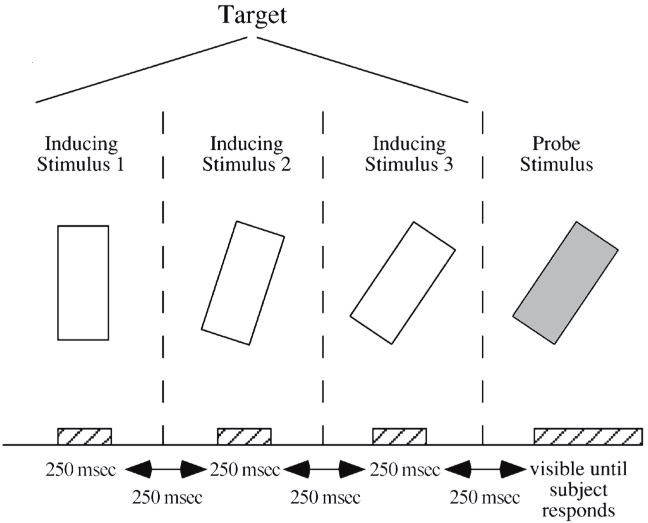
\includegraphics[width=80mm]{rm_a.png} &
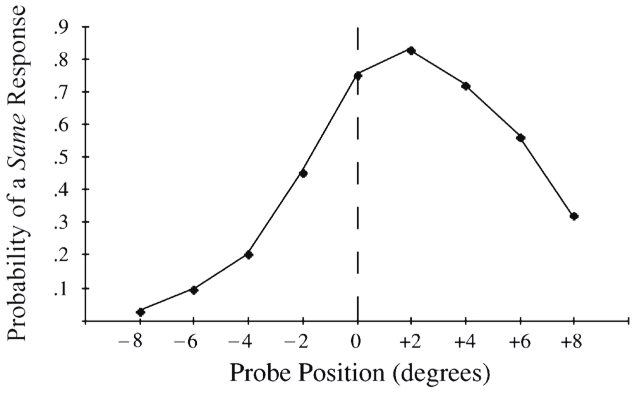
\includegraphics[width=80mm]{rm_b.png} \\
b) \\
\multicolumn{2}{c}{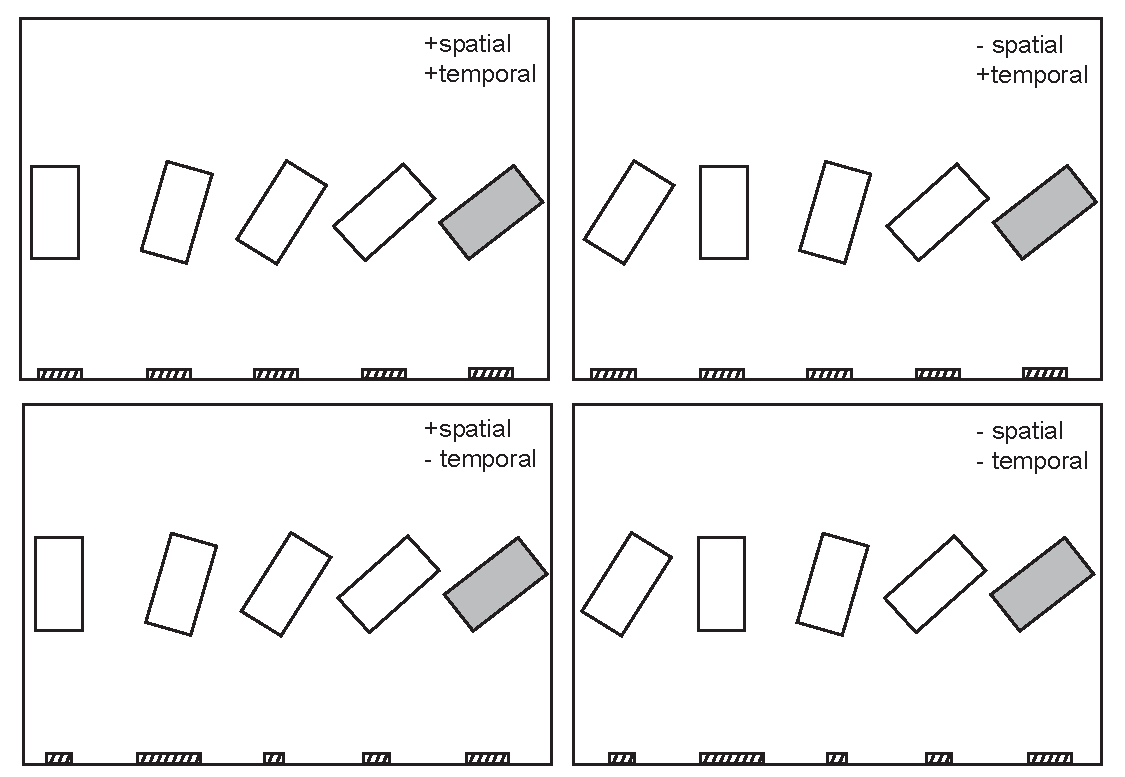
\includegraphics[width=140mm]{rm_mod.pdf}} \\
\end{tabular}
\caption{Representational momentum paradigm modified for spatiotemporal prediction.}
\label{fig:exp1_task}
\end{figure}

In the context of the LeabraTI theory, it is expected that rhythmic, temporal predictability, independent of the spatial properties of the stimulus, will induce changes in alpha-band power compared to arhythmic stimulus presentation. Spatial predictability, in contrast, should manifest as changes in gamma-band power, compared to randomized stimulus sequences. It is unclear whether these effects will have a multiplicative effect in the oscillatory domain (and if so, within what frequency band) or whether multiplicative effects are restricted to the ERP domain. More standard ERP analysis will be conducted on the probe stimulus itself to determine the replicability of \incite{DohertyRaoMesulamEtAl05} as well as to determine the basic effects of representational momentum on evoked potentials. Surprisingly, no work has investigated the neural correlates of representational momentum with EEG, so any positive effects would be a novel contribution to the literature.

\section{Experiment 2}
The spatial and temporal predictability of stimuli in Experiment 1 will be completely randomized. However, one interesting extension on the basic proposed paradigm is concerned with the learnability of pseudorandom spatial and temporal sequences and moreover and associated changes in alpha and gamma oscillations. Presumably, the visual system learns the deterministic event structure of the physical world in early development. Using pseudorandom spatiotemporal sequences will allow investigation of how the brain adapts to a novel event structure. This will be the focus of Experiment 2.

The basic design of Experiment 2 will be the same as Experiment 1, except that the spatial and temporal stimulus sequences will be pseudorandom and repeated throughout the experiment. It is anticipated that subjects will be able to at least partially learn these sequences over the course of a single experimental session during which EEG activity is recorded, but the experiment can be decomposed into multiple sessions if necessary with pre- and post-training tests during which EEG activity will be recorded. 

Gamma-band activity is expected to track the learned spatial predictability of pseudorandom stimulus sequences, with the result converging on that of the spatially deterministic conditions in Experiment 1. A firm prediction regarding the effect of sequence learning on alpha-band activity in this case is more difficult to make. Alpha-band coherence might track the temporal event structure of learned sequences, even for arrhythmic conditions. This effect would mirror the predicted gamma-band effect, but in the alpha frequency range, since temporal uncertainty would be reduced by learning. However, this effect might be unlikely given that alpha generally only entrains to rhythmic environmental events \cite{LakatosKarmosMehtaEtAl08,SchroederLakatos09}. Another possibility is that irregular inter-stimulus intervals could reset the phase of alpha \cite{LandauFries12,KlimeschSausengHanslmayr07,PalvaPalva07}, a property that would diminish as the brain learns when to anticipate the next stimulus in the inducing sequence. Phase-based analyses \abbrevcite[e.g.,]{MakeigWesterfieldJungEtAl02} will likely be necessary to determine the result of learning on temporal predictability.

Finally, it is also difficult to predict how spatial and temporal sequence learning will affect the representational momentum displacement effect. If multiple arbitrary events can indeed become associated, then it is not unlikely that there will be a displacement for a probed stimulus in the direction of the stimulus that associated with the next item in the spatiotemporal sequence. This is the general prediction of the LeabraTI theory, and is consistent with literature indicating that associations can be formed between arbitrary, unrelated stimuli \cite{Miyashita88,SakaiMiyashita91,MeyerOlson11}. On the other hand, the representational momentum displacement effect might be related specifically by the physical laws of the natural world \cite[e.g., spatiotemporal coherence, gravity, friction, etc., see]{Hubbard05}, and might be difficult to modify via associations that break these laws.

\section{Experiment 3}
Experiments 1 and 2 use relatively simple stimuli that vary across a single dimension (orientation) to elicit the representational momentum displacement effect. Previous work using the ``ball'' paradigm \cite{RohenkohlNobre11,DohertyRaoMesulamEtAl05}, including the simulations described in Chapter \ref{chap:leabrati}, also contained only univariate manipulations in stimulus position. However, as long as stimulus properties vary consistently across space and time, displacement should theoretically occur. It is somewhat surprising then, that very few studies have used complex, multidimensional stimuli to study representational momentum \cite[see][for one example that uses facial expressions]{YoshikawaSato08}. A related line of research has investigated the role of spatiotemporal coherence in recognition of 3D objects, with a number of experiments reporting  faster recognition and better memory for specific views when objects were learned in a spatially and temporally predictable manner, compared an unpredictable manner \cite{MitsumatsuYokosawa03,VuongTarr04,BalasSinha09b,WangZhang10}. These effects could be explained by generic spatial and temporal prediction mechanisms that feed into higher-level object processing circuits to drive learning in an self-supervised manner.

Experiment 3 will investigate the independent effects of learned spatial and temporal predictability on complex, 3D object stimuli. The basic design will be identical to Experiment 2, but with the addition of novel object stimuli to ensure that subjects are not already familiar with their geometrical structure. The objects will be rotated in the the x, y, and z planes and possibly translated and scaled as well. with The LeabraTI theory is agnostic about whether spatial predictability applies to unidimensional stimulus transformations (e.g., position, orientation, scale) or complex multidimensional transformations, and thus effects are expected to be congruent between Experiments 2 and 3 so long as the spatial and temporal properties are at least partially deterministic (i.e., pseudorandom).

Again, it is expected that gamma-band activity will track the learned structural predictability of 3D object sequences, just as it is expected to track the learned spatial predictability of stimulus sequences in Experiment 2. Alpha-band activity is also expected to follow the effect found in Experiment 2, either tracking the temporal intervals at which the object transformations occur or exhibiting phase-resetting behavior that diminishes once subjects are successful at predicting reliable temporal properties. The representational momentum displacement effect is similarly expected to be analogous to that of Experiment 2, if it is indeed a product of generic spatial and temporal prediction mechanisms.

\section{Modeling and simulation}
All experiments will be simulated using the model of V1 and V2 processing with the LeabraTI framework described in Chapter \ref{chap:leabrati}. The minus-plus phase cosine metric will be used to determine whether representational momentum displacement effects are due to prediction-sensation processes. It is expected that a larger cosine will translate to a shift in the curve depicted in Figure \ref{fig:exp1_task}a, providing a mechanistic explanation of the displacement. More advanced analyses may attempt to model the effects of spatial and temporal predictability on gamma-band activity. Alpha oscillations will not be explicitly modeled, as they are a fundamental assumption of the model and are necessary for its most basic operation. Instead, the LeabraTI theory simply predicts that alpha desynchronization is related to the brain's ability to predict when the next stimulus event will occur, which is possible when events are rhythmic.

Experiment 1 will be simulated by training the model with high spatial and temporal predictability stimulus sequences (Figure \ref{fig:exp1_task}b, top-left condition), emulating the deterministic event structure of the physical world. The minus-pluse phase cosine is expected to be maximal in this condition and will provide a baseline against which to compare the other conditions. The model will then be tested under the remaining three conditions: low spatial but high temporal predictability, high spatial but low temporal predictability, and low spatial and low temporal predictability. Simulations of the low spatial predictability conditions will contain randomized stimulus sequences. Since time in the LeabraTI implementation is discretized into 100 ms frames, simulations of the low temporal predictability conditions will be simulated by omitting stimulus inputs on some frames, capturing the basic variability in inter-stimulus intervals of experimental stimulus sequences. The cosine in these conditions is expected to be lower than baseline, with the lowest measure in the low spatial \textit{and} temporal predictability condition.

Experiment 2 will be simulated in a similar manner to Experiment 1, except that the model will be trained using pseudorandom stimulus sequences. In the context of the LeabraTI theory, this type of event structure is just as learnable as the sequences in Experiment 1 despite not conforming to the event structure of the physical world. Thus, it is expected that the model will be capable of learning these sequences to the same level of Leabra phase cosine similarity as in simulations of Experiment 1. These data will be fitted to match subjects' data to account for variance across subjects in how well-learned the sequences are. 

Experiment 3 is expected to produce results analogous to Experiments 1 and 2. The model of V1 and V2 processing might need to be augmented with more complex processing layers (e.g., V4, IT) to perform the spatial pooling necessary to predict multidimensional transformations. Preliminary simulations, however, indicate that greater than baseline predictability is possible with the current model.

\chapter{Experimental variants and general discussion}
\label{chap:variants}

The LeabraTI theory integrates a number of findings from the systems neuroscience literature to explain how the brain integrates information and uses it to predict subsequent events. Central to the theory are the roles of alpha and gamma oscillatory mechanisms, which are assumed to index temporal and spatial prediction mechanisms respectively. Alpha and gamma oscillations each have their own independent literatures, and they have been shown to interact with a variety of other mechanisms. In this chapter, I discuss variants of the experiments proposed in Chapter \ref{chap:experiments} that target these interactions, providing insight into different focal aspects of the broader LeabraTI theory. 

The proposed line of experiments as presently described is concerned with the brain's ability to learn to predict subsequent events in spatiotemporal sequences and how this process depends on and/or modulates alpha and gamma oscillatory mechanisms. It also asks whether spatial and temporal prediction are a more general processes that can operate on complex multidimensional stimuli, feeding the results into higher-level object-processing circuits to drive learning in a self-supervised manner. The proposed line of experiments should be preferred, as it is more well-defined at present, but the variants may replace one or more of the proposed experiments at the committee's discretion.

\section{Alpha oscillations, attentional periodicities, and phase resets} 
In the LeabraTI theory, alpha oscillations caused by Layer 5 (and possibly thalamic) neurons' rhythmic bursting are suggested to implement a pacemaking ``clock'' that updates at regular intervals, allowing the brain to anticipate ``when'' the next set of inputs should be expected. This process is implemented in the generic LeabraTI model as a discretization of time that updates predictions and sensations every 100 ms. Previous lines of research have been interested in whether perception and cognition are similarly discretized \cite{VarelaToroJohnEtAl81,VanRullenReddyKoch05,VanRullenKoch03b,VanRullenDubois11}. The picture painted in Chapter \ref{chap:leabrati} however is not one of discrete perception, but rather, periodic updating by specific neural subpopulations. These periodicities have been suggested to be influenced by a range of endogenous and exogenous events including attention and salience.

Attention has been shown to \textit{decrease} alpha-band power recorded by scalp EEG, which is associated with an \textit{increase} in perceptual sensitivity (\nopcite{BuschDuboisVanRullen09},\abbrevnopcite{MathewsonLlerasBeckEtAl11}). To explain this finding, various researchers have suggested that attention might allow perception to operate in a ``continuous mode'' with a longer duty cycle by synchronizing its periodicities with periodicities in the environment, minimizing loss of information \cite{SchroederLakatos09,JensenBonnefondVanRullen12}. Salient events in the environment also have an effect on alpha oscillations, but in terms of their phase. Specifically, salient events such as visual cues reset the phase of ongoing alpha oscillations \cite{LandauFries12}. Cross-modality cues from the auditory events can also reset the phase of ongoing alpha oscillations over visual cortex \cite{RomeiGrossThut12}. What function might these phase resets have? One possibility is that phase-resetting reflects an attentional orienting response, so that as soon as resources are focused on the new, salient stimulus, perception can operate optimally in a continuous mode. 

Thus, the proposed experiments might benefit from additional manipulations involving attention or salient events that cause phase resetting. For example, the experimental display could potentially be divided two hemifields with a distractor task (e.g., target detection) that either occurred in the same hemifield as the representational momentum task (i.e., valid cue) or the opposite (i.e., invalid cue). This attentional manipulation alone is likely to increase the size of any potential effects since it forces perception into a periodic mode. Additionally it might provide a triple dissociation between temporal prediction, spatial prediction, and spatial attention.

Phase coherence was already suggested in Chapter \ref{chap:experiments} as a potential analysis to determine how well the brain could anticipate pseudorandom temporal events. However, it might also be fruitful to examine the effects of unexpected events that attract attention away from the representational momentum task. A number of experiments have indicated that auditory stimuli can modulate distortion effects \cite{ShamsKamitaniShimojo02,TeramotoHidakaGyobaEtAl10,ChienOnoWatanabe13}, but virtually no experiments have investigated the neural correlates of these illusions with EEG. Alpha oscillatory phase resetting with unexpected auditory events could modulate learning depending on when they occur with respect to the next event in the psuedorandom sequence (i.e., the stimulus onset asynchrony, or SOA). An SOA of 50 ms would likely discourage learning since the phase reset would cause the next event to be experienced during the brain's prediction of what happens next (i.e., Leabra minus phase), making it difficult to generate a proper sensory prediction error signal. An SOA of 100 ms, on the other hand, might accelerate learning as it would place the brain in the optimal state to both make a prediction and experience the subsequent sensory event, driving generation of the sensory prediction error signal.

\section{Gamma oscillations, and predictive coding} 
In the LeabraTI theory, gamma oscillations reflect the convergence of afferent and efferent interareal synapses onto superficial neurons, which result in a non-pacemaking, higher overall rate of activity. Layer 6 $\rightarrow$ Layer 4 $\rightarrow$ Layer 2/3 transthalamic and/or direct feedforward connections as well as Layer 6 $\rightarrow$ Layer 2/3 feedback connections (Figure \ref{fig:objrec_ti}a) leverage the previous moment's context to drive a prediction about what happens next in superficial layers. The LeabraTI theory is agnostic about the relative contributions of feedforward and feedback interareal connections in driving the prediction, but an alternative theory of prediction -- predictive coding (\nopcite{RaoBallard97}; \abbrevnopcite{BastosUsreyAdamsEtAl12}; \nopcite{ArnalGiraud12}) -- specifically posits that feedback connections are responsible for the prediction. Predictive coding is also centered around the position that neurons encode sensory prediction errors (i.e., a difference-based encoding), opposed to sensory events and predictions themselves. Specifically, predictions conveyed via feedback connections are compared with sensory inputs to generate the the sensory prediction error, which is what is actually encoded by neurons and relayed downstream where the process is repeated. This type of representation is efficient, since only the residual differences between sensations and predictions are encoded (opposed to both in the LeabraTI model), but requires inhibitory feedback to perform the difference-based computation between sensations and predictions. This requirement is at odds with biological feedback, which has been shown to be fundamentally excitatory (\nopcite{Roland10}, but see also \nopcite{Spratling08}).

There are several experimental variants that might shed light on the actual coding scheme used in the brain. Because predictive coding is suggested to depend on interareal feedback, it can potentially be disrupted by backward masking \cite{WyatteCurranOReilly12,LammeRoelfsema00,DiLolloEnnsRensink00}. A mask presented with the proper SOA would block the prediction error computation due to a mismatch between the feedback prediction (coding the stimulus) and feedforward sensation (coding the mask). However, the time course of predictive coding is not well-defined, so a given mask SOA (e.g., 100 ms) might either interfere with the prediction error computation, or with other mechanisms such as the LeabraTI theory's temporal context updating, making this particular variant somewhat nondiagnostic. 

One alternative might be to focus the variant on hypotheses regarding the nature of the prediction error. Predictive coding theory suggests that if predictions perfectly match sensations, then the neural response will be attenuated since residual prediction error is minimized. However, many experiments indicate that successful prediction actually enhances neural responses \cite{DohertyRaoMesulamEtAl05,EstermanYantis10}. A recent experiment by \abbrevincite{KokRahnevJeheeEtAl12} has attempted to resolve this conflict by suggesting that experiments often confound prediction with attention, and when properly controlled, unattended stimuli elicit neural responses in agreement with a reduction in prediction error. However, when stimuli are attended, feedforward sensations are differentially weighted, resulting in a reversal of prediction error reduction, producing the enhancement effect often observed experimentally. This experimental variant involving attention dovetails nicely with the one described in the previous section, and would provide insight into the oscillatory effects of attention on prediction-sensation processes. Furthermore, the fine-grained temporal resolution of EEG might make it possible to parcel out the relative contributions of prediction and sensation in ERP waveforms to determine their relative weightings as well as their overall time course.

\section{Remaining miscellany}
One remaining point worth mentioning concerns the choice of behavioral task in the proposed experiments. The representational momentum paradigm was originally chosen because it is a unified experimental framework that could be integrated with the unidimensional shape stimuli used in Experiments 1 and 2 as well as the complex multidimensional object stimuli in Experiment 3. However, the probe-based nature of the task (Figure \ref{fig:exp1_task}a) adds additional complexity, especially when combined factorially with the four experimental conditions of interest (Figure \ref{fig:exp1_task}b), which might create difficulty in achieving statistical power levels necessary to compare EEG and oscillatory effects. This issue, however, might be partially addressable by sampling only key probe orientations (e.g., 0, +2, and +4 degrees). If one of the variants described in this chapter replaces one or more of the proposed experiments, the experimental task can also be changed, mitigating this issue.

One attractive alternative is to simply use the ``ball'' paradigm \cite{RohenkohlNobre11,DohertyRaoMesulamEtAl05} since it has already been linked to prediction in the alpha-band. It has also already been simulated using the model of V1 and V2 processing described in Chapter \ref{chap:leabrati}. These points suggest that the experiments and simulations have a high probability of working compared to the representational momentum paradigm, which has surprisingly never been investigated using EEG. However, changing experimental paradigms prevents investigation of spatial and temporal prediction mechanisms on complex multidimensional object stimuli, making it unclear whether any potential effects would generalize to real-world stimuli. It also cuts ties to my previous line of research centered around object recognition \cite{WyatteCurranOReilly12,OReillyWyatteHerdEtAl13,WyatteHerdMingusEtAl12}. Determining the best experimental paradigm and variants will be the goal of the proposal meeting.

\newpage
\bibliographystyle{apa}
\bibliography{ccnlab}
\end{document}